\documentclass[conference]{IEEEtran}
\IEEEoverridecommandlockouts
\usepackage{amsmath,amssymb}   % amssymb also provides \checkmark and loads amsfonts
\usepackage{graphicx}
\usepackage{textcomp}
\usepackage{xcolor}
\usepackage{booktabs}
\usepackage{enumitem}
\usepackage{array}
\usepackage{float}             % needed for [H] placement
\usepackage{listings}
\usepackage{csquotes}          % recommended by biblatex

\lstset{
  basicstyle=\ttfamily\footnotesize,
  breaklines=true,
  columns=fullflexible,
  frame=single
}

\setlist{nosep,leftmargin=*}

% Status tags
\newcommand{\done}{\textcolor{green!40!black}{\textbf{[$\checkmark$ Done]}}}
\newcommand{\wip}{\textcolor{orange!70!black}{\textbf{[$\circ$ In progress]}}}
\newcommand{\planned}{\textcolor{blue!60!black}{\textbf{[$\square$ Planned]}}}
% Red TODO notes; remove every \todo before submission (search for "\todo").
\newcommand{\todo}[1]{\par\noindent\textcolor{red}{\textbf{TODO:} #1}\par}

\usepackage[style=ieee, backend=biber]{biblatex}
\addbibresource{../references.bib}

\title{Topic Modeling of Autonomous Vehicle News Coverage Across Publications, 2016--2020\\
\large Progress Report 3
}

\author{\IEEEauthorblockN{Lauren Gamber }
\IEEEauthorblockA{\textit{Department of Mathematical Sciences} \\
\textit{Montana State University}\\
Bozeman, MT \\
Lauren.Gamber@montana.edu}
\and
\IEEEauthorblockN{Laura Banaszewski}
\IEEEauthorblockA{\textit{Gianforte School of Computing} \\
\textit{Montana State University}\\
Bozeman, MT \\
laura.banaszewski@montana.edu}
\and
\IEEEauthorblockN{Mary Kate Carara}
\IEEEauthorblockA{\textit{Department of Mathematical Sciences} \\
\textit{Montana State University}\\
Bozeman, MT \\
connellymarykate@gmail.com}
}

\date{Due: November 8th, 2026}

\begin{document}

\maketitle

\newpage

\begin{center}\large\textbf{Response to Feedback}\end{center}

This report addresses each comment on Progress Report 2:
\begin{itemize}
    \item \textbf{Answers to research question(s)} The results section now includes approved topic labels, representative articles, publication comparisons, and examples of how the models split and combine themes. BERTopic has higher coherence, while LDA has higher keyword diversity and assigns every article.
    \item \textbf{Testing decisions} The completed 80/20 split is an exploratory robustness check. Configuration and stopword development used the full corpus before the split, so it is not a completely isolated test set.

\end{itemize}
Major changes since Progress Report 2: completed model comparison and robustness checks, 110 approved interpretive labels, and a new corpus audit correcting the unsupported clean-audit claim.

\begin{center}\large\textbf{Implementation Progress and Findings}\end{center}

Since Progress Report 2, both selected pipelines have been fit to the same 7,332 articles. Comparison naming, publication comparisons, seed and configuration checks, a shared-period comparison, and an exploratory split are complete. The remaining analytical dependency is the independent human-fit review.

\textbf{Classical pipeline configuration.}  For the classical pipeline, we chose a K of 40 during previous exploratory work. For this progress report, we explored configuration choices for \texttt{max\_iter}, document topic prior, and topic word prior. 

To select a value for \texttt{max\_iter}, we fit LDA with K=40 at seed 42 with a \texttt{max\_iter} of 10, 25, 50, 100, 200, and evaluated the training perplexity for each. We select the smallest value after which iterations changed perplexity by less than 1\%, as such a small change indicates convergence. 

From 50 iterations to 100 iterations, we observed a decrease in perplexity of 0.53\% (3240.8-3223.7), indicating that a \texttt{max\_iter} of 50 is sufficient. 

\begin{table}[ht]
\centering
\caption{Training perplexity of LDA ($K=40$, seed 42) at increasing iteration caps. The last column is the relative improvement over the previous setting.}
\label{tab:max-iter}
\begin{tabular}{rrr}
\hline
\texttt{max\_iter} & Perplexity & Change from previous (\%) \\
\hline
10  & 3451.6 & --- \\
25  & 3283.9 & 4.86 \\
50  & 3240.8 & 1.31 \\
100 & 3223.7 & 0.53 \\
200 & 3216.6 & 0.22 \\
\hline
\end{tabular}
\end{table}

To select the document-topic prior ($\alpha$) and the topic-word prior ($\eta$), we fixed $K = 40$, \texttt{max\_iter} $= 50$, and the random seed at 42. We tuned the two priors one at a time, holding the other fixed, and evaluated each of the values $\{0.01, 0.025, 0.1, 0.5\}$. For each fitted model, we extracted the top 10 terms of every topic and scored the model on coherence ($c_v$), keyword diversity, and perplexity.

We selected values by coherence and keyword diversity, and report perplexity for reference. Perplexity was reported but not used for selection, since it correlates poorly with human judgments of topic quality (TODO: add reference) and was computed on the training data.

\begin{table}[ht]
\centering
\caption{LDA results for the document-topic prior $\alpha$ ($K=40$, \texttt{max\_iter}~$=50$, seed 42, $\eta$ at its default). Coherence is mean $c_v$ over topics; diversity is the fraction of unique terms among the top 10 terms of all topics; dominant probability is the mean over articles of the highest topic probability.}
\label{tab:alpha}
\begin{tabular}{rrrrr}
\hline
$\alpha$ & Coherence ($c_v$) & Diversity & Perplexity & Mean dominant prob. \\
\hline
0.01  & 0.650 & 0.695 & 3279 & 0.452 \\
0.025 & 0.652 & 0.705 & 3241 & 0.450 \\
0.1   & 0.655 & 0.710 & 3246 & 0.438 \\
0.5   & 0.657 & 0.748 & 3378 & 0.361 \\
1.0   & 0.636 & 0.787 & 3458 & 0.293 \\
\hline
\end{tabular}
\end{table}

For the document topic prior, we selected selected $\alpha = 0.1$. Coherence was effectively tied across $\alpha \in [0.01, 0.5]$, and fell only at $\alpha = 1.0$ (the largest value scikit-learn permits). Because coherence did not provide a clear selection, we made our decision based on mean dominant-topic probability, since our analysis assigns each article to its highest-probability topic and compares these assignments with BERTopic. This value decreased steadily as $\alpha$ increased. Larger values such as $\alpha = 0.5$ improved keyword diversity (0.710 to 0.748) but reduced the mean dominant probability from 0.438 to 0.361. We therefore chose $\alpha = 0.1$, which retains near-maximal coherence and the highest assignment confidence among the settings that match the best coherence, while remaining close to the scikit-learn default of $1/K = 0.025$.

With a 

\begin{table}[ht]
\centering
\caption{LDA results for the topic-word prior $\eta$ ($K=40$, \texttt{max\_iter}~$=50$, seed 42, $\alpha = 0.1$). Coherence is mean $c_v$ over topics; diversity is the fraction of unique terms among the top 10 terms of all topics; dominant probability is the mean over articles of the highest topic probability.}
\label{tab:eta}
\begin{tabular}{rrrrr}
\hline
$\eta$ & Coherence ($c_v$) & Diversity & Perplexity & Mean dominant prob. \\
\hline
0.01  & 0.650 & 0.708 & 3304 & 0.435 \\
0.025 & 0.655 & 0.710 & 3246 & 0.438 \\
0.1   & 0.642 & 0.743 & 3319 & 0.459 \\
0.5   & 0.600 & 0.815 & 3626 & 0.578 \\
1.0   & 0.578 & 0.720 & 3937 & 0.618 \\
\hline
\end{tabular}
\end{table}

We selected $\eta = 0.025$, which is also the scikit-learn default of $1/K$. With $\alpha$ fixed at 0.1, coherence was highest at this value ($c_v = 0.655$) and declined for larger $\eta$ (0.642 at $\eta = 0.1$, 0.600 at $\eta = 0.5$, and 0.578 at $\eta = 1.0$). Larger values of $\eta$ increased the mean dominant-topic probability (from 0.438 to 0.618) and, up to $\eta = 0.5$, keyword diversity, but both gains came with lower coherence. 

\begin{center}\large\textbf{Remaining Work}\end{center}
\begin{itemize}
    \item Complete independent article-fit reviews and calculate rating summaries and reviewer agreement. \wip
    \item Integrate those results and revise the discussion if they change the current interpretations. \planned
\end{itemize}


\begin{center}\large\textbf{Paper Outline 3}\end{center}
\noindent\emph{Status legend:} \done~completed;
\wip~started, partially complete; \planned~not yet started.

\section*{Abstract}
Autonomous vehicle (AV) news coverage was extensive between 2016 and 2020, but the themes it emphasized, and whether they differ across publications, remain poorly characterized. We apply two topic modeling pipelines to 7,332 AV-related articles from 25 publications in the ``All the News'' dataset~\cite{mckinley2021}: a Latent Dirichlet Allocation (LDA) baseline and BERTopic, which embeds articles with GTE-small, reduces dimensionality with UMAP, and clusters them with HDBSCAN. We evaluate both pipelines with $c_v$ topic coherence, keyword diversity, seed stability, and topic overlap. On the deduplicated corpus, LDA produced 40 topics with mean $c_v=0.6552$, and BERTopic produced 70 topics with mean $c_v=0.7047$, leaving 18.04\% of articles unassigned. Approved interpretive labels identify deployment, safety, litigation, and policy themes, alongside mixed and format-driven topics. Selected publication differences persist across models and coverage checks, but their magnitudes depend on topic definitions and some LDA comparisons change across seeds. These results provide a matched comparison of how model choice changes the themes identified in AV coverage.

\section*{Introduction}
In recent years, autonomous vehicles (AVs) have received extensive news coverage spanning technological development, safety, regulation, and commercial usage. Because news coverage shapes how the public perceives emerging technologies~\cite{christen2007media, anania2018effects}, understanding what this coverage emphasizes matters for researchers, policymakers, and the public. However, AV coverage spans many news outlets and consists of large volumes of unstructured text, making recurring themes difficult to identify. Topic modeling is a method that can identify those themes. 

Recent work has applied topic modeling to AV news~\cite{kang2025unveiling}, but two questions remain open. Prior analyses pooled articles across outlets, so it
is unknown whether publications differ in which themes they emphasize. In addition, no study has applied classical and embedding-based topic models to the same AV news corpus, so it is unclear whether the reported themes depend on the
choice of model. We address these gaps with three research questions:

\begin{itemize}
    \item What themes characterize news coverage of autonomous vehicles from 2016 to 2020?
    \item How does the prevalence of these themes differ across publications?
    \item How does the choice of topic model affect the themes identified?
\end{itemize}

We apply LDA and BERTopic to 7,332 AV-related articles from 25 publications in the All the News dataset~\cite{mckinley2021}. We contribute (i) the first topic-model-based comparison of AV coverage across individual U.S. publications and (ii) a matched evaluation of LDA and BERTopic on the same corpus, testing how the choice of model changes the themes identified.


\section*{Related Work}
News media are a major source of information about emerging technologies and can shape public perceptions \cite{christen2007media}. For autonomous vehicles (AVs), this influence appears to start with the headline: Anania et al.~\cite{anania2018effects} found that participants who read positive article titles reported greater willingness to ride in a driverless vehicle than those who read negative ones.

Penmetsa et al.~\cite{penmetsa2023news} measured sentiment in U.S. AV news coverage but did not identify themes. Jelinski et al.~\cite{jelinski2021undifferentiated} examined themes, but only in German coverage. Neither study applies topic modeling.

Bakalos et al.~\cite{bakalos2020} studied public opinion of autonomous transportation using sentiment analysis of social media posts. This work shows how the public feels about AVs but does not identify which themes news coverage emphasizes.

Topic modeling can identify those themes. Classical models such as Latent Dirichlet Allocation (LDA)~\cite{blei2003lda} represent each article as a mixture of topics and each topic as a word distribution. LDA infers topics from how words co-occur in articles. LDA assumes a bag-of-words model, meaning it forms topics without considering word order. Non-negative matrix factorization (NMF)~\cite{lee1999nmf} is another classical topic modeling technique that factors a document-term matrix. These classical models are very interpretable and inexpensive to run. However, they ignore context, and the number of topics has to be chosen in advance. 

Embedding-based models instead represent articles using pretrained language models. BERTopic~\cite{grootendorst2022bertopic} is one of the most widely known embedding-based models. It embeds articles, reduces dimensionality with UMAP~\cite{mcinnes2018umap}, clusters articles with HDBSCAN~\cite{campello2013hdbscan}, and describes each cluster with class-based TF-IDF~\cite{alammar2024}. An advantage of this type of topic modeling is that the embeddings capture context, so BERTopic can group articles with similar meaning even when they use different words. Additionally, the number of topics comes from clustering. However, BERTopic assigns each article to only one topic and is more computationally expensive. 

The study closest to ours is Kang et al.~\cite{kang2025unveiling}, who applied BERTopic to 11,708 AV-related news articles published between 2002 and 2021 in the ProQuest ABI/INFORM database. By analyzing paragraphs pooled across outlets, they identified 45 AV topics, showing that the AV news coverage extends beyond safety and performance to battery supply chains, regulatory uncertainty, and infrastructure. 

Kang et al. pooled paragraphs from all sampled outlets, so their results do not investigate whether different publications emphasize different themes. Additionally, no study has fit classical and embedding-based topic models to the same AV news corpus. Because classical and embedding-based topic models differ in interpretability, stability, and cost, it is unclear whether the identified themes reflect model choice or the true topics of AV news coverage. 

Our study addresses both gaps. We compare autonomous vehicle news themes across 25 publications and apply an LDA pipeline and a BERTopic pipeline to the same corpus of news articles.


\section*{Data}
Our research utilizes the ``All the News'' dataset \cite{mckinley2021}, available freely on Kaggle. We downloaded the dataset in September of 2026. The full dataset includes 2.79 million English news articles from January 2016 to April 2020. We used a regular expression to identify a subset of 7,337 articles. The subset covers 25 publications from January 1, 2016, through March 26, 2020. Each observation represents one article. The articles are copyrighted news text used for research only, and the only personal data is author bylines.

% Body
\begin{figure}[H]
\centering
\begin{lstlisting}
self[- ]driving|driverless|autonomous (car|vehicle|truck|driving)|robo[- ]?taxi|waymo|tesla'?s? autopilot
\end{lstlisting}
\caption{Case-insensitive regular expression used to identify AV-related articles.}
\label{fig:regex}
\end{figure}

The CSV contains 15 columns: article ID, an additional source index, date, year, month, day, author, title, article body, URL, section, publication, title match, body hits, and word count. Article bodies will be the modeling input; publication and date will be metadata for interpreting and comparing results. There is no supervised target variable, so the data does not have labels or class distribution; topics are discovered rather than predicted.

An initial audit identified missing author and section values and five duplicate article bodies, with no missing article bodies or publications. Both pipelines use the same documented article set and duplicate-handling policy: for articles with duplicate bodies, the earliest-dated article is retained and the others are dropped, bringing the article total to 7,332. Since author and section are not used for our analysis, we retained articles missing this data.

We manually reviewed a random sample of 30 articles (seed 42) for relevance, boilerplate, and malformed text. Of the 30 articles, 24 were centrally relevant, five peripheral, and one not relevant. Seven contained boilerplate; four had malformed text and two had uncertain malformed-text judgments. These categories overlap: nine articles had at least one present boilerplate or malformed-text judgment. These sample findings correct the earlier unsupported claim of a uniformly clean audit; they do not establish corpus-wide defect rates. The fitted corpus was not changed.

\begin{table}[H]
\caption{Corpus summary by publication after duplicate removal (N = 7,332 articles). Word counts are article medians.}
\label{tab:corpus}
\centering
\footnotesize
\setlength{\tabcolsep}{3pt}
\begin{tabular}{lrrcr}
\toprule
\textbf{Publication} & \textbf{Articles} & \textbf{\%} & \textbf{First--Last} & \textbf{Med. words} \\
\midrule
TechCrunch          & 1,214 & 16.6 & 2016-01--2020-03 & 433 \\
CNBC                &   977 & 13.3 & 2016-01--2020-03 & 456 \\
Reuters             &   854 & 11.6 & 2016-01--2020-03 & 419 \\
The Verge           &   830 & 11.3 & 2016-01--2020-03 & 505 \\
Mashable            &   554 &  7.6 & 2016-01--2020-03 & 403 \\
The New York Times  &   501 &  6.8 & 2016-01--2020-03 & 1,014 \\
Vox                 &   500 &  6.8 & 2016-01--2020-02 & 678 \\
Axios               &   360 &  4.9 & 2017-01--2019-12 & 326 \\
The Hill            &   353 &  4.8 & 2016-01--2020-02 & 737 \\
Wired               &   249 &  3.4 & 2016-01--2020-03 & 614 \\
Gizmodo             &   215 &  2.9 & 2016-01--2019-09 & 496 \\
Business Insider    &   200 &  2.7 & 2016-02--2020-03 & 653 \\
Other (13 pubs.)    &   525 &  7.2 & 2016-01--2020-03 & 691 \\
\midrule
\textbf{Total}      & \textbf{7,332} & \textbf{100} & 2016-01--2020-03 & 496 \\
\bottomrule
\end{tabular}
\end{table}

The regular expression is shown in Fig.~\ref{fig:regex}. Table~\ref{tab:corpus}
shows uneven coverage: the four largest publications contribute 52.9\% of
articles, while 13 publications together contribute 7.2\%. Article length is
right-skewed (median 496, mean 761, maximum 28{,}048 words), which motivates
chunked embeddings.

\begin{figure}[H]
\centering
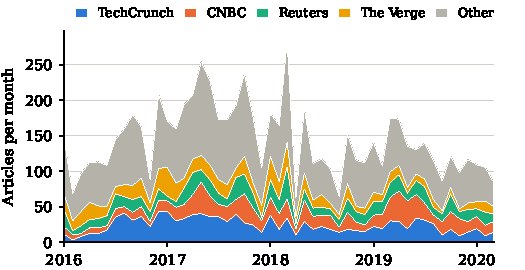
\includegraphics[width=\columnwidth]{figures/monthly_articles.pdf}
\caption{Monthly AV article counts after duplicate removal (N = 7,332), stacked by publication. The four largest publications are shown separately; the remaining 21 are grouped as Other. March 2020 is a partial month (through March 26).}
\label{fig:monthly}
\end{figure}

Monthly volume is also uneven (Fig.~\ref{fig:monthly}). Coverage peaks in 2017 and early 2018, with a maximum of 283 articles in March 2018, and then declines to roughly 100--150 articles per month. The largest peaks are split roughly evenly between the four largest publications and the remaining 21, so they reflect corpus-wide spikes rather than a single outlet. Because individual months can be dominated by a few stories, we treat short-lived topics with caution when comparing publications.

For feature construction, the classical pipeline (LDA) uses unigram bag-of-words counts, whereas BERTopic uses lightly cleaned full text for embeddings and unigram counts for keywords.

\section*{Methodology}
\subsection*{Classical Pipeline (LDA)}
The classical pipeline follows four stages \cite{qamar2024}: (1) data preprocessing, (2) document-term representation, (3) topic model fitting, and (4) topic interpretation. We tokenize article bodies, remove English and custom stopwords, and build a document-term count matrix. LDA provides an interpretable baseline through its topic-word distributions and article-level topic mixtures.

Tokenization was performed by (1) merging words with apostrophes and hyphens, (2) deleting non-ASCII characters, (3) dropping words with fewer than three characters, and (4) lowercasing all words.

After removing scikit-learn's English stopwords, number-only tokens, and tokens shorter than three characters, we ranked the remaining tokens by document frequency and inspected the top 100. We removed 40 reporting and filler terms (e.g., \textit{said}, \textit{told}, \textit{according}, \textit{thats}) and 10 terms that appear in 53--88\% of articles because they define the corpus (e.g., \textit{selfdriving}, \textit{autonomous}, \textit{car}, \textit{company}); the full list is in Table~\ref{tab:stopwords}. Custom stopword removal reduced the median article length from 264 to 227.5 tokens (mean 391.5 to 339.6; range 70--11,986 to 56--10,353).

\begin{table}[H]
\caption{Custom stopwords removed for the LDA pipeline, chosen from the 100 tokens with the highest document frequency.}
\label{tab:stopwords}
\centering
\footnotesize
\begin{tabular}{@{}p{0.22\columnwidth}p{0.72\columnwidth}@{}}
\toprule
\textbf{Group} & \textbf{Terms} \\
\midrule
Reporting and filler (40) & said, says, say, told, according, like, just, thats, dont, did, going, think, lot, right, way, make, making, use, used, using, need, want, come, able, called, including, big, long, far, better, end, number, new, time, year, years, week, today, early, earlier \\
\addlinespace
Corpus-defining or generic (10) & selfdriving, autonomous, cars, car, vehicles, vehicle, company, companies, companys, technology \\
\bottomrule
\end{tabular}
\end{table}

Once tokenization was complete, we represented each article as unigram counts (not TF-IDF), using scikit-learn's \texttt{CountVectorizer}. We kept terms that appear in at least 5 articles (\texttt{min\_df}$=5$) and in no more than 50\% of articles (\texttt{max\_df}$=0.5$). The resulting document-term matrix had 21,528 terms and is 98.97\% sparse (221 distinct terms per article on average), falling within the expected sparsity range for news articles.

Using scikit-learn's \texttt{LatentDirichletAllocation}, we fit and scored models with $K\in\{10,20,30,40,50,60,70\}$ topics using seed 42 and \texttt{max\_iter}$=20$. We selected $K=40$ by weighing $c_v$, perplexity, and diversity, and by manually reviewing selected topics. 

\textbf{Model.} LDA~\cite{blei2003lda} treats each article $d$ as a mixture of $K$ topics and each topic $k$ as a distribution over the vocabulary:
\begin{equation}
\begin{gathered}
\theta_d \sim \mathrm{Dir}(\alpha), \qquad \phi_k \sim \mathrm{Dir}(\eta),\\
z_{dn} \sim \mathrm{Mult}(\theta_d), \qquad w_{dn} \sim \mathrm{Mult}(\phi_{z_{dn}}),
\end{gathered}
\label{eq:lda}
\end{equation}
where $z_{dn}$ is the topic of the $n$th word $w_{dn}$ in article $d$. An article's dominant topic is $\arg\max_k \hat{\theta}_{dk}$, where $\hat{\theta}_d$ is its inferred topic mixture.

\textbf{Implementation.} We use scikit-learn's \texttt{LatentDirichletAllocation}, which approximates the posterior with batch variational Bayes (\texttt{learning\_method='batch'}). The $K$ grid used \texttt{max\_iter}$=20$; the final $K=40$ model uses \texttt{max\_iter}$=100$, chosen after testing 20, 50, and 100 iterations. The priors are fixed at scikit-learn's symmetric defaults, $\alpha=\eta=1/K$, rather than learned. Fitting and scoring each $K$ in the grid with seed 42 is implemented, as is the seed-stability check (seeds 7 and 21, compared by ARI). Computing $\hat{\theta}_d$ with the fitted model's \texttt{transform}, dominant-topic assignment, and topic labeling are planned.

\textbf{Rationale.} LDA is our baseline for three reasons. Its topic-word distributions and article-level mixtures are directly interpretable, and unlike BERTopic it lets an article belong to several topics. It is the standard reference model in topic-modeling comparisons, including the original BERTopic evaluation~\cite{grootendorst2022bertopic}. 

\subsection*{Modern Pipeline (BERTopic)}
The modern pipeline follows five stages \cite{alammar2024, kumari2026}: (1) data preprocessing, (2) document embedding, (3) dimensionality reduction, (4) document clustering, and (5) topic representation and interpretation.

\textbf{Document embedding.} GTE-small~\cite{li2023gte} accepts at most 512 tokens. We tokenize each article's full text with the model's tokenizer and split it into consecutive, non-overlapping chunks of at most 480 tokens. Each chunk is wrapped in the model's start and end tokens and embedded separately, giving chunk vectors $\mathbf{v}_{d1},\dots,\mathbf{v}_{dJ}\in\mathbb{R}^{384}$ with token counts $n_{d1},\dots,n_{dJ}$. The article embedding is the token-weighted mean of its chunk vectors, scaled to unit length:
\begin{equation}
\bar{\mathbf{v}}_d = \frac{\sum_{j=1}^{J} n_{dj}\,\mathbf{v}_{dj}}{\sum_{j=1}^{J} n_{dj}}, \qquad
\mathbf{e}_d = \frac{\bar{\mathbf{v}}_d}{\lVert\bar{\mathbf{v}}_d\rVert_2}.
\label{eq:pooling}
\end{equation}
The model revision is pinned, and embeddings are cached so that every configuration uses identical vectors.

\textbf{Reduction and clustering.} UMAP~\cite{mcinnes2018umap} reduces the embeddings to 5 dimensions (cosine metric, \texttt{min\_dist}$=0$), because density-based clustering degrades in high dimensions. HDBSCAN~\cite{campello2013hdbscan} then clusters the reduced vectors (Euclidean metric, \texttt{min\_samples}$=10$, excess-of-mass cluster selection). HDBSCAN infers the number of topics from the data rather than requiring it in advance, and places articles that fit no dense cluster in an outlier class ($-1$) instead of forcing them into a topic.

\textbf{Topic representation.} To describe each topic, BERTopic concatenates the articles assigned to a cluster $c$ into one class document and scores each term $t$ with class-based TF-IDF~\cite{grootendorst2022bertopic}:
\begin{equation}
W_{t,c} = \mathrm{tf}_{t,c}\cdot\log\!\left(1+\frac{A}{f_t}\right),
\label{eq:ctfidf}
\end{equation}
where $\mathrm{tf}_{t,c}$ is the frequency of $t$ in class $c$ (normalized by the class's total term count), $f_t$ is the frequency of $t$ across all classes, and $A$ is the average number of terms per class. A topic's keywords are its ten highest-weighted terms. Counts use unigrams, English stopwords removed, from a fixed vocabulary learned once from the individual articles with \texttt{min\_df}$=5$: a term must appear in at least five articles. Learning the vocabulary before concatenation keeps the threshold defined over articles rather than over class documents, and the same vocabulary is reused across configurations. Keyword tokenization matches the reference corpus used for coherence, so every topic term can be scored.

\textbf{Selected configuration.} We compared UMAP neighbor counts of 15 and 30 with HDBSCAN minimum cluster sizes of 25, 50, and 100. After reviewing coherence, topic sizes, keywords and representative articles, we selected 30 neighbors and a minimum cluster size of 25 at seed 42. We then reviewed the resulting 70 labels.

\subsection*{Implementation Environment}
Both pipelines run in Python 3.13, with dependency versions pinned by a \texttt{uv} lockfile: bertopic 0.17.4, sentence-transformers 6.1.0, umap-learn 0.5.12, hdbscan 0.8.44, scikit-learn 1.9.1, and gensim 4.4.0 (used for $c_v$ coherence). Experiments run on an Apple-silicon Mac under macOS; GTE-small embeddings are computed on the GPU through PyTorch's Metal Performance Shaders (MPS) backend, and all other stages run on the CPU. Code, the corpus manifest, and run outputs are available at \url{https://github.com/laurengamber/DataMiningProject}.

\section*{Experimental Design}
\begin{enumerate}
    \item \textbf{Select configurations and label topics.} We considered $c_v$ coherence~\cite{roder2015coherence}, topic sizes, keywords, and representative articles when selecting one configuration per pipeline. Configurations and labels will be finalized before independent human evaluation. Final evaluation articles and duplicate copies will be excluded from development review and topic naming.
    \item \textbf{Independent human evaluation.} Two reviewers will independently rate the same 100 articles, sampled once with seed 42 before topic labels are finalized, on a 1--5 scale for how well the assigned topic describes the article, separately for each model. We will report exact agreement (the share of identical ratings), agreement within one point, and quadratic-weighted Cohen's $\kappa$, which penalizes large disagreements more heavily than near-misses on the ordinal scale. Articles that BERTopic leaves unassigned will be reported separately and excluded from $\kappa$. A 95\% bootstrap interval for $\kappa$ (1,000 resamples of articles) will quantify uncertainty given the small sample.
    \item \textbf{Compare topics across publications.} For each pipeline, we calculated the proportion of each publication's articles assigned to each topic. Heat maps and representative articles identify shared themes and differences in thematic emphasis. We report publication sample sizes, include BERTopic's unassigned category, and interpret differences descriptively, considering unequal date coverage.
    \item \textbf{Compare pipeline outputs.} We compared coherence, keyword diversity, computational cost, and topic overlap; human ratings remain pending. We also examined whether both methods support similar conclusions about publication differences, accounting for differences in topic granularity. Success means identifying article-supported themes, characterizing their prevalence across publications, and explaining how these findings depend on the model.
    \item \textbf{Assess robustness.} We repeated selected configurations at seeds 7 and 21 and examined all six BERTopic configurations. A coverage-based restriction to 2016--2018 retained 4,931 articles from 11 publications with at least 20 articles in each year. This comparison restricts existing assignments rather than refitting temporal models. Vice and Vice News remain separate publications.
\end{enumerate}

\textbf{Data splitting.} Because the goal is to describe a fixed corpus rather than to predict labels, the final models were fit on all 7,332 articles. An exploratory 80/20 split, drawn within each publication/year group with seed 42, gave 5,866 training and 1,466 held-out articles, and ten single-article groups remained in training. Vocabularies and models were fit on training articles only, with fixed settings and cached pretrained embeddings. We computed held-out perplexity for LDA, $c_v$ against the same held-out reference for both pipelines, and held-out topic assignments using each model's \texttt{transform}. However, configuration and stopword development preceded the split and used the full corpus. This is not untouched final-test performance, and near-duplicate stories may cross partitions. The separate 100-article human sample evaluates within-corpus article--label fit.

\textbf{Coherence.} We will measure topic coherence with $c_v$~\cite{roder2015coherence}, computed with gensim's \texttt{CoherenceModel}, using each topic's ten highest-weighted unigrams. Word and word-pair probabilities are estimated from a boolean sliding window of 110 tokens over a reference corpus. Each top word is represented by a vector of its normalized pointwise mutual information (NPMI) with all ten top words, and a topic's $c_v$ is the mean cosine similarity between each word's vector and the vector of the full top-word set (indirect confirmation). Both pipelines use the same reference corpus: every modeled article, stripped of non-alphanumeric characters, lowercased, and tokenized with scikit-learn's English-stopword analyzer. Top words missing from the reference vocabulary are dropped before scoring, and BERTopic's outlier class ($-1$) is excluded. Per-topic values and their mean are saved, and all top words in both selected models were covered by the reference vocabulary.

\textbf{Topic alignment.} To compare topics across pipelines, we represent each topic by the set of its ten highest-weighted terms. For every pair of an LDA topic $A$ and a BERTopic topic $B$, we compute the Jaccard similarity
\begin{equation}
J(A,B) = \frac{|A\cap B|}{|A\cup B|},
\label{eq:jaccard}
\end{equation}
which ranges from 0 (no shared terms) to 1 (identical term sets). BERTopic's outlier class is excluded. The resulting heat map and best keyword matches are saved as supporting material. Shared article assignments provide a separate comparison of topic boundaries in Fig.~\ref{fig:split-merge}.

\section*{Results}
\textbf{Purpose:} Present the themes, publication patterns, and pipeline comparison supported by the completed analysis.

\textbf{Planned content:} 
\begin{itemize}
    \item \textbf{Topic keywords, labels, sizes and representative articles} We reviewed and selected 40 comparison-specific LDA names and 70 BERTopic names. Table~\ref{tab:selected-topics} gives paired examples and representative articles. Both models recover Waymo deployment, Uber--Waymo litigation, and congressional legislation. Both also assign the same 27 articles to Hill.TV interview coverage, a source-associated format rather than necessarily a distinct AV theme. \done
    \item \textbf{Topic proportions across publications, one heat map per pipeline, alongside publication sample sizes}Figure~\ref{fig:publication-examples} shows selected examples using all articles from each outlet as the denominator, including BERTopic outliers. The Verge's Waymo share exceeds TechCrunch's in both selected models (6.14\% versus 3.05\% for LDA; 9.28\% versus 7.00\% for BERTopic). Vox's litigation share exceeds Reuters' (9.40\% versus 5.04\%; 8.80\% versus 4.33\%). The Hill's congressional share is 33.99\% under LDA but 8.22\% under BERTopic; Wired's urban-mobility share is 14.06\% versus 2.01\%. These are illustrative corpus comparisons, not rankings of all outlet output. \done
    \item \textbf{Quantitative and human evaluations, with a comparison table of metrics, human ratings, and computational cost} Table~\ref{tab:model-comparison} reports coherence, diversity, and seed stability. BERTopic has higher coherence, while LDA has higher keyword diversity and assigns every article. LDA's mean dominant probability is 0.4382, and 68.71\% of articles have a maximum probability below 0.5, so dominant-topic summaries discard substantial mixture information. Human-fit results remain pending. \wip
    \item \textbf{Agreement and differences between pipelines in themes and publication patterns} Figure~\ref{fig:split-merge} shows LDA's Uber testing/crash topic divided among several BERTopic event clusters. Conversely, BERTopic's Tesla topic combines articles from LDA's product and crash-investigation topics. More topics do not imply finer distinctions everywhere. \done
    \item \textbf{Robustness and uncertainty checks} The Waymo and litigation directions above persist across all six BERTopic configurations and the shared-period subset. LDA's seed-7 litigation match reverses the Vox--Reuters ordering (4.20\% versus 4.45\%). LDA's Waymo direction persists, but matched clusters are broader. The shared-period restriction preserves the substantial model differences for The Hill and Wired. \done
    \item \textbf{Exploratory split} Held-out-reference $c_v$ is 0.6130 for LDA and 0.6337 for BERTopic. LDA's held-out perplexity is 6,922.24. BERTopic leaves 30.97\% of held-out articles unassigned, compared with 23.37\% in training. \done
\end{itemize}

\begin{figure}[H]
\centering
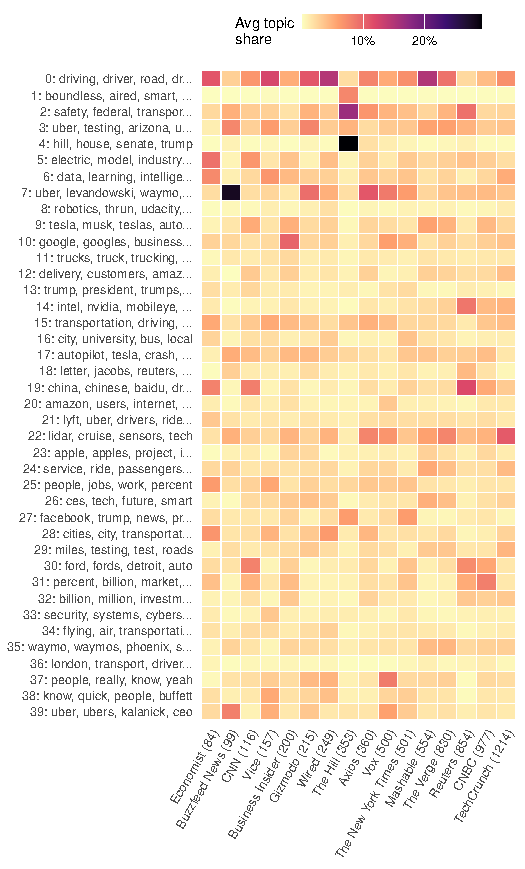
\includegraphics[width=\columnwidth]{figures/heatmap_lda_column.pdf}
\caption{Average LDA topic proportions by publication ($K = 40$, N = 7,332). Each cell is the mean topic share of that publication's articles; article counts are in parentheses. Only the 16 publications with at least 50 articles are shown, and Vice and Vice News are combined.}
\label{fig:lda-heatmap}
\end{figure}

\begin{table}[H]
\centering
\caption{\label{tab:lda-topics}LDA topics and sizes}
\centering
\fontsize{7}{9}\selectfont
\begin{tabular}[t]{r>{\raggedright\arraybackslash}p{3.8cm}rrr}
\toprule
Topic & Label & Articles & \% docs & Avg \%\\
\midrule
0 & driving, driver, road, drivers & 685 & 9.3 & 7.1\\
22 & lidar, cruise, sensors, tech & 511 & 7.0 & 5.9\\
2 & safety, federal, transportation, rules & 431 & 5.9 & 4.8\\
7 & uber, levandowski, waymo, ubers & 409 & 5.6 & 4.8\\
3 & uber, testing, arizona, ubers & 356 & 4.9 & 4.3\\
19 & china, chinese, baidu, driving & 345 & 4.7 & 3.8\\
14 & intel, nvidia, mobileye, driving & 290 & 4.0 & 3.3\\
9 & tesla, musk, teslas, autopilot & 257 & 3.5 & 3.0\\
30 & ford, fords, detroit, auto & 224 & 3.1 & 3.0\\
35 & waymo, waymos, phoenix, service & 211 & 2.9 & 2.6\\
6 & data, learning, intelligence, machine & 201 & 2.7 & 3.0\\
31 & percent, billion, market, revenue & 201 & 2.7 & 2.9\\
5 & electric, model, industry, market & 198 & 2.7 & 2.7\\
10 & google, googles, business, team & 198 & 2.7 & 3.2\\
17 & autopilot, tesla, crash, driver & 192 & 2.6 & 2.9\\
12 & delivery, customers, amazon, nuro & 187 & 2.6 & 2.3\\
28 & cities, city, transportation, parking & 176 & 2.4 & 2.1\\
29 & miles, testing, test, roads & 173 & 2.4 & 2.5\\
24 & service, ride, passengers, rides & 171 & 2.3 & 2.8\\
15 & transportation, driving, driverless, industry & 166 & 2.3 & 3.1\\
39 & uber, ubers, kalanick, ceo & 156 & 2.1 & 2.1\\
26 & ces, tech, future, smart & 141 & 1.9 & 2.3\\
27 & facebook, trump, news, president & 141 & 1.9 & 1.8\\
37 & people, really, know, yeah & 132 & 1.8 & 2.6\\
4 & hill, house, senate, trump & 131 & 1.8 & 2.0\\
23 & apple, apples, project, iphone & 130 & 1.8 & 1.5\\
25 & people, jobs, work, percent & 121 & 1.7 & 2.1\\
11 & trucks, truck, trucking, otto & 111 & 1.5 & 1.3\\
32 & billion, million, investment, raised & 106 & 1.4 & 2.0\\
21 & lyft, uber, drivers, ridehailing & 83 & 1.1 & 1.7\\
16 & city, university, bus, local & 70 & 1.0 & 1.4\\
18 & letter, jacobs, reuters, information & 67 & 0.9 & 1.5\\
34 & flying, air, transportation, drones & 67 & 0.9 & 1.2\\
38 & know, quick, people, buffett & 61 & 0.8 & 1.7\\
33 & security, systems, cybersecurity, military & 53 & 0.7 & 0.9\\
20 & amazon, users, internet, cloud & 50 & 0.7 & 1.1\\
13 & trump, president, trumps, campaign & 49 & 0.7 & 1.0\\
8 & robotics, thrun, udacity, students & 32 & 0.4 & 0.7\\
1 & boundless, aired, smart, hilltvs & 27 & 0.4 & 0.5\\
36 & london, transport, driverless, trial & 22 & 0.3 & 0.6\\
\bottomrule
\end{tabular}
\end{table}


\begin{table*}[t]
    \centering
    \caption{Selected interpretive labels, counts, top keywords and representative articles. LDA names annotate unchanged classical topics; BERTopic names come from the selected modern label table. Examples are outside the independent fit-review sample. Complete inventories remain supporting material.}
    \label{tab:selected-topics}
    \footnotesize
    \setlength{\tabcolsep}{4pt}
    \begin{tabular}{lp{0.40\textwidth}rlc}
    \toprule
    Model/topic & Interpretive label & Articles & Keywords & Example \\
    \midrule
    LDA 35 & Waymo driverless-service rollout & 211 & waymo, waymos, phoenix & \cite{example2340111} \\
    BERTopic 1 & Waymo autonomous-driving development and deployment & 438 & waymo, waymos, krafcik & \cite{example546719} \\
    LDA 7 & Uber-Waymo trade-secret litigation & 409 & uber, levandowski, waymo & \cite{example61037} \\
    BERTopic 2 & Uber-Waymo trade-secret litigation & 334 & levandowski, uber, waymo & \cite{example1341648} \\
    LDA 4 & Congressional AV legislation & 131 & hill, house, senate & \cite{example1861945} \\
    BERTopic 20 & Congressional AV legislation & 85 & legislation, senate, safety & \cite{example2490394} \\
    LDA 1 & Hill.TV Boundless technology interview coverage & 27 & boundless, aired, smart & \cite{example1819183} \\
    BERTopic 67 & Hill.TV Boundless technology interview coverage & 27 & boundless, aired, hilltvs & \cite{example1814127} \\
    \bottomrule
    \end{tabular}
    \end{table*}
    
    \begin{table}[ht]
    \centering
    \caption{Selected models on the same 7,332 articles. BERTopic excludes the outlier class from topic metrics. All top words are covered by the common coherence reference.}
    \label{tab:model-comparison}
    \footnotesize
    \begin{tabular}{lrr}
    \toprule
    Measure & LDA & BERTopic \\
    \midrule
    Topics & 40 & 70 \\
    Assigned articles & 7,332 & 6,009 \\
    Mean $c_v$ & 0.6552 & 0.7047 \\
    Keyword diversity & 0.7100 & 0.6514 \\
    Seed-7 ARI & 0.3230 & 0.9614 \\
    Seed-21 ARI & 0.3469 & 0.9760 \\
    Independent human fit & Pending & Pending \\
    \bottomrule
    \end{tabular}
    \par\smallskip
    \raggedright ARI uses all 7,332 articles for LDA, but only the 5,697/5,678 assigned in both runs for BERTopic at seeds 7/21. BERTopic outlier-status agreement is 91.04\%/91.13\%; the ARIs therefore have different evaluation populations.
    \end{table}
    
    \begin{figure*}[t]
    \centering
    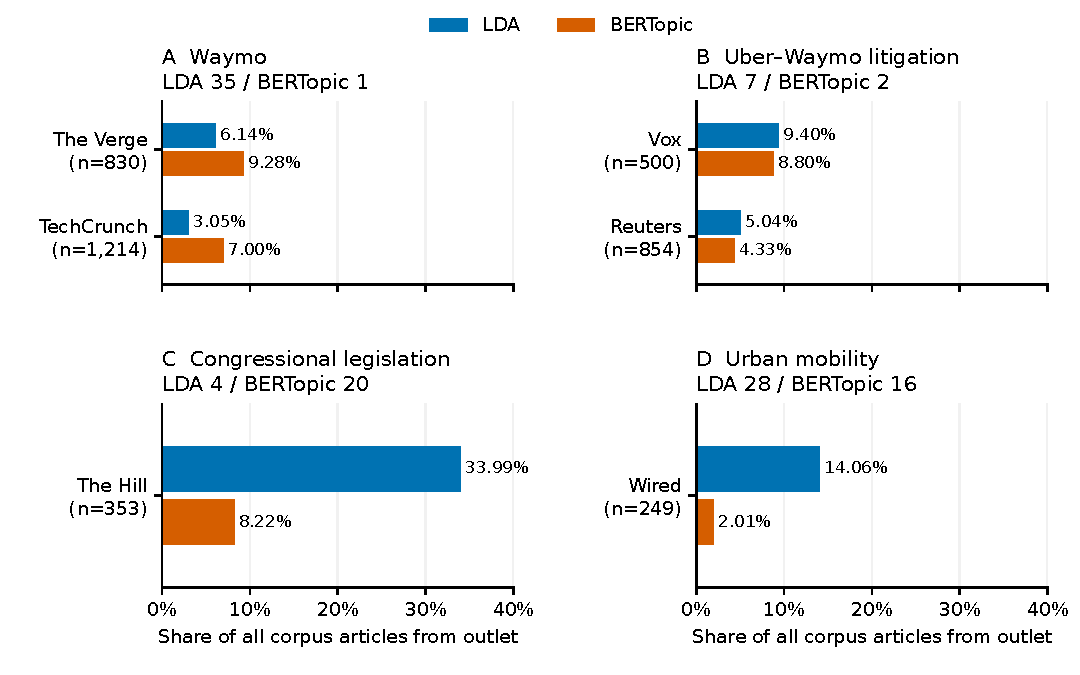
\includegraphics[width=0.90\textwidth]{../code/modern-methods/Results/robustness/2026-11-26/report_selection/publication_examples.pdf}
    \caption{Dominant-topic shares for four illustrative themes. Shares use all corpus articles from each publication, including BERTopic outliers; $n$ gives the publication denominator. Panels share a percentage scale, but topic breadth differs across models. The Vox--Reuters litigation ordering reverses under LDA seed 7.}
    \label{fig:publication-examples}
    \end{figure*}
    
    \begin{figure*}[t]
    \centering
    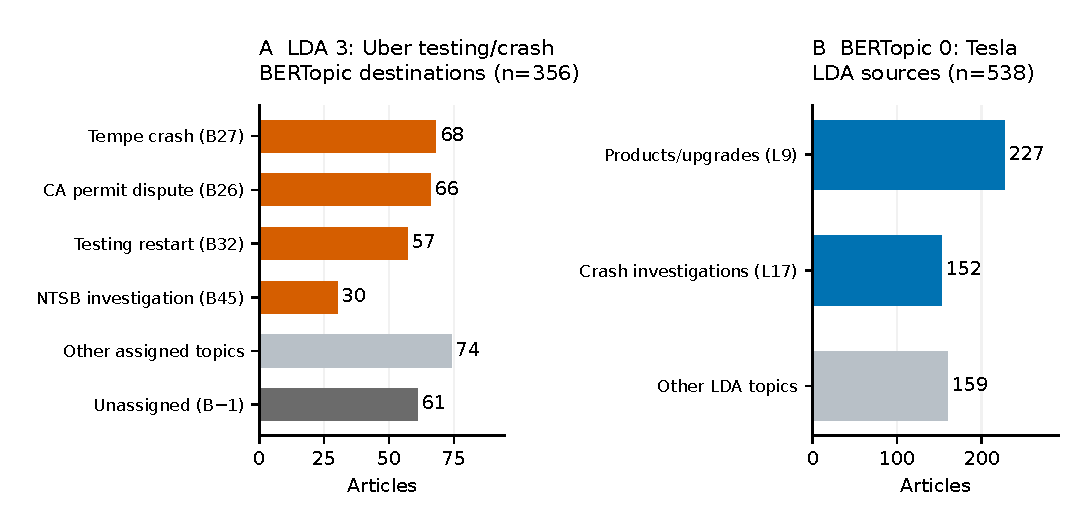
\includegraphics[width=0.90\textwidth]{../code/modern-methods/Results/robustness/2026-11-26/report_selection/topic_split_merge.pdf}
    \caption{Cross-model article overlap. Panel A partitions all 356 articles in LDA topic 3 across BERTopic destinations, including 61 unassigned articles. Panel B partitions all 538 articles in BERTopic topic 0 across LDA topics. The panels have different denominators and count scales. Article overlap describes topic boundaries, not model accuracy or causal flow.}
    \label{fig:split-merge}
    \end{figure*}

    \textbf{Supporting evidence:} complete topic inventories, publication heat maps, the Jaccard matrix, seed/configuration matching, and split results are saved with the analysis.

\section*{Human Review}
\textbf{To do: Ordinal Regression}



\section*{Discussion}
\textbf{Purpose:} Interpret the identified themes and publication differences in relation to the research questions, modeling choices, and prior work on AV news coverage.

\textbf{Planned content:} 
\begin{itemize}
    \item \textbf{Interpretation of shared themes and differences in thematic emphasis across publications} The interpretation identifies business, technology, safety, and policy themes alongside source and format effects. Publication comparisons are conditional on topic definitions, sampled articles, and the robustness checks. \done
    \item \textbf{Influence of pipeline choice on substantive findings} LDA and BERTopic give complementary descriptions: they recover some shared themes but split and combine article groups differently. The metrics do not establish an overall accuracy winner. \done
    \item \textbf{Relationship to prior AV media research} Compare the recurring themes with the 45 topics reported by Kang et al.~\cite{kang2025unveiling}, accounting for their paragraph-level analysis, different period, and different corpus. \planned
    \item \textbf{Implications of evaluation results} Independent fit ratings are needed before drawing conclusions about how well approved labels describe individual articles. \planned
    \item \textbf{Discussion of robustness and uncertainty} Discuss the LDA litigation reversal, changing topic breadth, BERTopic outliers, and the exploratory split. \planned 
    \item \textbf{Potential extensions and future work} Consider sensitivity to boilerplate removal, relevance filtering, and near-duplicate handling without treating these unperformed changes as part of the current fitted analysis. \planned
\end{itemize}

\textbf{Required evidence and figures:} the Results tables and figures; themes will be compared with the 45 topics reported by Kang et al.~\cite{kang2025unveiling}. No new figures are planned.

\section*{Limitations and Responsible Use Considerations}
The corpus may not represent all AV news coverage. Keyword filtering may omit relevant articles or retain irrelevant ones, while syndicated stories may overrepresent particular themes. Unequal publication sizes and date coverage limit comparisons, especially for publications with few articles. Major news events may also produce temporary concentrations of coverage that do not reflect sustained thematic emphasis.

Both pipelines depend on preprocessing and modeling choices. LDA's dominant-topic summaries simplify articles containing multiple themes, while BERTopic's embeddings, chunk pooling, and clustering settings may affect topic boundaries and leave articles unassigned. Robustness checks will assess these effects. Human evaluation by two team members provides a limited, subjective assessment.

\section*{Conclusion}
\textbf{Purpose:} Summarize the findings about AV news themes and publication differences, explain the contribution of comparing modeling pipelines, and identify remaining work.

\textbf{Planned content:} 
\begin{itemize}
    \item Main themes and differences across publications \wip
    \begin{itemize}
        \item Business themes: Waymo deployment, Uber testing/crash, congressional legislation
        \item Technology themes: Tesla product, crash investigation, urban mobility
        \item Safety themes: NHTSA investigation, Tesla crash, Uber testing/crash
        \item Policy themes: congressional legislation, NHTSA regulation, Tesla product
    \end{itemize}
    \item Influence of pipeline choice on findings \wip
    \begin{itemize}
        \item LDA and BERTopic give complementary descriptions: they recover some shared themes but split and combine article groups differently. The metrics do not establish an overall accuracy winner.
    \end{itemize}
    \item Remaining analysis and future work \wip
    \begin{itemize}
        \item Independent fit ratings are needed before drawing conclusions about how well approved labels describe individual articles.
        \item Consider sensitivity to boilerplate removal, relevance filtering, and near-duplicate handling without treating these unperformed changes as part of the current fitted analysis.
    \end{itemize}
\end{itemize}

\textbf{Required evidence and figures:} summarizes the Results and Discussion; no tables or figures are planned.

\newpage
\section*{References}
\printbibliography[heading=none]

\end{document}